\section{\color{red}Tekstalgoritmer}
	Generelt problem: Vi er interesserte i å finne ut om en streng er en substreng av en annen streng. Vi kaller substringen for en nål $i$, av lengde $m$, og stringen for en høystakk $h$, av lengde $n$.

	\subsection{Brute force}
		Brute force-metoden er som navnet tilsier ikke spesielt gjennomtenkt: Til å begynne med sjekker vi hver karakter i høystakken mot den første i nåla. Hvis vi har likhet sjekker vi det neste tegnet i høystakken mot det neste i nåla. Vi fortsetter slik til vi enten finner hele nåla i høystakken eller til vi har ulikhet, og i så fall fortsetter vi med å sjekke det neste tegnet i høystakken mot det første i nåla.

	\subsubsection{Analyse}
		Worst case så får vi mismatch $(n-m)$ ganger og suksess $(n-m)+1$ ganger, Totale sammenligninger er $((n-m)+1\times m)$ som gir kjøretid $O(n^2)$.

	\subsection{\color{red}Boyer-Moore}
		Dette er en rask substringalgoritme. Med Boyer-Moore preprosserer vi nåla før vi begynner å søke. Vi regner ut hvor mange hopp vi kan gjøre for hvert enkelt tegn i nåla ved mismatch. Dette er bad character shift. Good character shift også... Algoritmen starter med å sjekke halen på nåla og ved eventuell match beveger seg mot venstre. Fortsetter så enten til hele nåla er matchet eller til mismatch, hvor vi i så fall beveger oss \verb|badShift[i]| bortover.

	\subsubsection{\color{red}Bad character shift}
		Vi beregner avstand til neste gang nål er på linje med høystakk\ref{huffman}.
	\subsubsection{\color{red}Good suffix shift}
		Vi bruker antall match før mismatch for å finne skip-avstand.

	\subsection{\color{red}Huffmankoding}\label{huffman}
		Huffmankoding er en måte å kode informasjon på, her tekst, på en måte der vi ikke mister noe informasjon (\textit{lossless}). Prinsippet går ut på å se på frekvensen til tegnene som forekommer, og gi kort kode til de tegnene som forekommer ofte, og lang kode til de som forekommer sjelden. Dette kan vi gjøre slik at vi har prefiksegenskapen intakt: Ingen koder er et prefiks av noen andre. Kodealfabetet \{9, 55\} har prefiksegenskapen, men \{9, 5, 59, 55\} har ikke. Måten Huffmankoding beholder denne egenskapen blir fort tydelig når vi ser på algoritmen. Kort fortalt er grunnen at vi benytter binære trær til å finne kodene.
		
		Algoritmen:
		\begin{enumerate}
			\item Lag frekvenstabell for alle tegn som forekommer i teksten.
			\item Betrakt hvert tegn som en node som skal settes sammen til et tre, og legg alle noder i en prioritetskø (heap. Se \ref{heap}) $P$.
			\item Mens $P$ har mer enn ett element:
				\begin{itemize}
					\item[-] Ta ut de to minste nodene fra $P$.	
					\item[-] Gi disse to en foreldernode med vekt lik summen av de to nodene.	
					\item[-] Legg foreldrenoden inn i $P$.	
				\end{itemize}
				Når dette er ferdig har vi et binært tre. Merk at det finnes svært sjeldent et entydig tre!
			\item Vi leser koden til et tegn ved å følge stien fra rotnoden ned til tegnets løvnode. Vi får en `0' når vi går til venstre, og en `1' når vi går til høyre. (Dette fungerer selvfølgelig ved å gjøre motsatt, så lenge man er konsekvent.) Merk igjen at det svært sjelden finnes entydige koder, men med denne algoritmen vil de uansett være optimale.
		\end{enumerate}
		Algoritmen burde bli klar når vi ser på et eksempel.

		\subsubsection{Eksempel på Huffmankoding}
		Anta at vi har en tekst ``BACADAEAFABBAAAGAH''. Vi setter opp en frekvenstabell for bokstavene i koden.
			\begin{center}
				\begin{tabular}{c c c}
					Tegn & Frekvens \\
					\hline
					A & 9\\
					B & 3\\
					C & 1\\
					D & 1\\
					E & 1\\
					F & 1\\
					G & 1\\
					H & 1
				\end{tabular}
			\end{center}
			Vi ser at vi kan parvis slå sammen to og to av nodene som har vekt 1: Vi slår sammen C og D, E og F, og G og H. Nå har (CD), (EF) og (GH) alle vekt 2. Vi slår så sammen B og (CD) til en node (B, CD) med vekt 5, og vi slår sammen (EF) og (GH) til en node (EF, GH) med vekt 4. Vi slår så igjen sammen (B, CD) og (EF, GH) slik at de får en foreldrenode med vekt 9. Til slutt slår vi sammen denne med noden A. Det resulterende treet er:

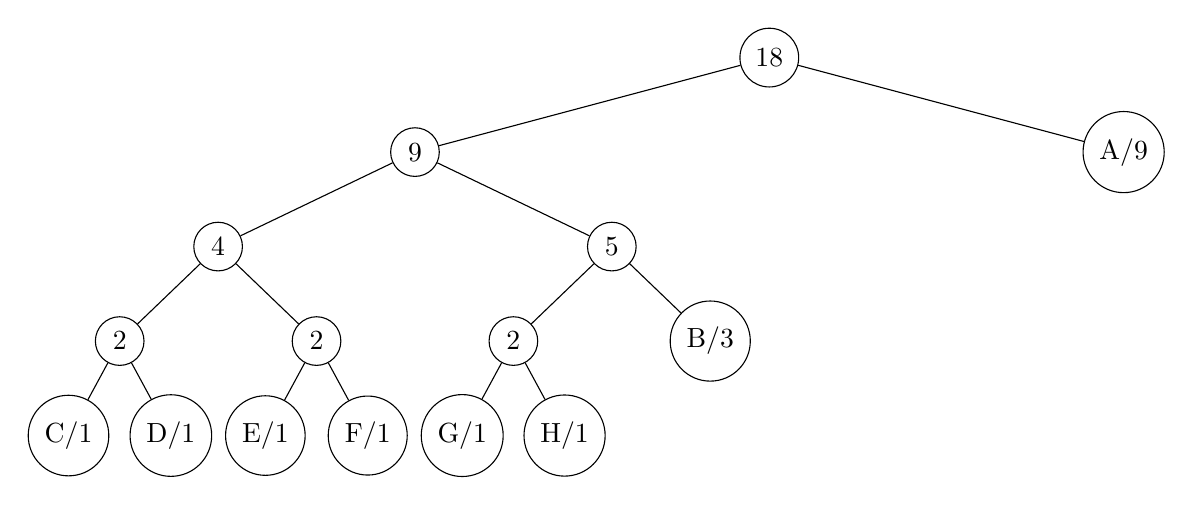
\begin{tikzpicture}[level distance=1.2cm,
level 1/.style={sibling distance=9cm},
level 2/.style={sibling distance=5cm},
level 3/.style={sibling distance=4cm},
level 3/.style={sibling distance=2.5cm},
level 4/.style={sibling distance=1.3cm}
]
\tikzstyle{every node}=[circle,draw]

\node {18}
    child {
	    node {9} 
	    child {
	    	node {4}
	    	child { node {2}
	    	child {node {C/1}}
	    	child {node {D/1}}}
	    	child { node {2}
	    	child {node {E/1}}
	    	child {node {F/1}}}
	    }
	    child {
	    	node {5}
	    	child { node {2}
	    	child {node {G/1}}
	    	child {node {H/1}}}
	    	child { node {B/3}
	    	}
	    }
		}
	child {
    node {A/9}
	}
;
\end{tikzpicture}

			Hvis vi nå følger regelen fra algoritmen om å skrive `0' når vi går venstre og 1 når vi går høyre ser vi at vi får kodene:
			\begin{center}
				\begin{tabular}{c c c}
					Tegn & Frekvens & Kode \\
					\hline
					A & 9 & 1\\
					B & 3 & 011\\
					C & 1 & 0000\\
					D & 1 & 0001\\
					E & 1 & 0010\\
					F & 1 & 0011\\
					G & 1 & 0100\\
					H & 1 & 0101
				\end{tabular}
			\end{center}
			Vi kan lett sjekke at prefiksegenskapen er intakt.
